%======================================================%
%   Beamer Presentation
%   LaTeX Template
%   compile using PDFTeXify, PDFLaTeX or XeLaTeX
%======================================================%

%--------------------------------------------------------------------------------
%   PACKAGES AND THEMES
%--------------------------------------------------------------------------------

\documentclass[notheorems,11pt,compress]{beamer}

\mode<presentation>{

%------- Beamer theme ------
\usetheme{CambridgeUS}
%\usetheme{Madrid}
%\usetheme{Boadilla}
%\usetheme{Frankfurt}
%\usetheme{Warsaw}
%\usetheme{Montpellier}


%------- Color theme ------
\usecolortheme{rose}
%\usecolortheme{orchid}
%\usecolortheme{lily}
%\usecolortheme{whale}
%\usecolortheme{dolphin}
%\usecolortheme{seahorse}

%\usetheme{boxes}
%\setbeamercovered{transparent}
%\usefonttheme[onlymath]{serif}
\usefonttheme{serif}
\usefonttheme{professionalfonts}

%\setbeamertemplate{headline}{}
%\setbeamertemplate{footline}{}
\setbeamertemplate{blocks}[rounded][shadow=true]
\setbeamertemplate{navigation symbols}{}
\setbeamertemplate{itemize items}[circle]  % ball, circle
\setbeamertemplate{enumerate items}[default]
%\setbeamertemplate{section in toc}[square]

}


%--------- 宏包  ----------
\usepackage[UTF8,noindent]{ctex}
%\usepackage[english]{babel}
\usepackage{amsmath,amssymb,version}
\usepackage{graphicx,fancybox,mathrsfs,multirow}
\usepackage{booktabs}
\usepackage{epsfig,epstopdf}
\usepackage{url,hyperref}
\usepackage{tabularx,array,makecell}
\usepackage{color,xcolor}
\usepackage{cases}
\usepackage{mathtools}
\usepackage{tikz}

%---------- 定义行距 ----------
%\renewcommand{\baselinestretch}{1.15}

%---------- 定义表格新命令 ----------
\newcolumntype{P}[1]{>{\centering \arraybackslash}p{#1}}
\newcolumntype{L}{X}
\newcolumntype{C}{>{\centering \arraybackslash}X}
\newcolumntype{R}{>{\raggedleft \arraybackslash}X}


%---------- 设置字体  ----------
\setbeamerfont{normal text}{family=\rmfamily}
\setbeamerfont{frametitle}{family=\rmfamily}
\setbeamerfont{title}{family=\rmfamily}
\setbeamerfont{subtitle}{family=\rmfamily}
\setbeamerfont{institute}{family=\kaishu}
\setbeamerfont{author}{family=\kaishu}
%\setbeamerfont{date}{family=\rmfamily}
\setbeamerfont{footline}{family=\kaishu}
\setbeamerfont{headline}{family=\sffamily}
\setbeamerfont{section in toc}{family=\rmfamily}
\setbeamerfont{subsection in toc}{family=\rmfamily}
\AtBeginDocument{\usebeamerfont{normal text}}


\setbeamertemplate{caption}[numbered]
\numberwithin{figure}{section}
\numberwithin{table}{section}
\numberwithin{equation}{section}

%---------- 定理设置  --------------
\setbeamertemplate{theorems}[numbered]
%\newtheorem{theorem}{Theorem}
\newtheorem{theorem}{定理}
\numberwithin{theorem}{section}
%\newtheorem{definition}{Definition}
\newtheorem{definition}{定义}
\numberwithin{definition}{section}
%\newtheorem{lemma}{Lemma}
\newtheorem{lemma}{引理}
\numberwithin{lemma}{section}
%\newtheorem{proposition}{Proposition}
\newtheorem{proposition}{命题}
\numberwithin{proposition}{section}
%\newtheorem{corollary}{Corollary}
\newtheorem{corollary}{推论}
\numberwithin{corollary}{section}
\theoremstyle{example}
%\newtheorem{example}{Example}
\newtheorem{example}{例}
%\numberwithin{example}{section}
\renewenvironment{proof}[1][证明]{\textbf{#1}:~~}{\qed\par}
\newenvironment{solution}{\par\noindent\textbf{解}:~~}{\par}

%---------- 调节公式的间距 ----------
%\AtBeginDocument{
%	\setlength{\abovedisplayskip}{4pt plus 1pt minus 1pt}
%	\setlength{\belowdisplayskip}{4pt plus 1pt minus 1pt}
%	\setlength{\abovedisplayshortskip}{2pt}
%	\setlength{\belowdisplayshortskip}{2pt}
%	\setlength{\arraycolsep}{2pt}
%}


%---------- 重新定义标题页 ----------
\makeatletter
\def\defmajor{}
\def\defstudy{}
\def\defadvisor{}
\newcommand{\major}[1]{\def\defmajor{#1}}
\newcommand{\study}[1]{\def\defstudy{#1}}
\newcommand{\advisor}[1]{\def\defadvisor{#1}}
\makeatother

\defbeamertemplate*{title page}{customized}[1][]{
\begin{center}
  {\makebox[160pt][s]{\bfseries\large\number\year\,届硕士学位论文答辩}}\\[2em]
  {\color[rgb]{0.50,0.00,0.00}\parbox[t]{10cm}{\Large\bfseries\centering \inserttitle}}\\[2em]
  \begin{tabular}{p{64pt}@{}c}
  \makebox[4em][s]{\kaishu 答辩人}~:&{\kaishu \insertauthor}\\[2pt]
  \makebox[4em][s]{\kaishu 专业}~:&{\kaishu \defmajor}\\[2pt]
  \makebox[4em][s]{\kaishu 指导教师}~:&{\kaishu \defadvisor}\\[2pt]
  \makebox[4em][s]{\kaishu 研究方向}~:&{\kaishu \defstudy}\\[2pt]
\end{tabular}
\vskip 2em
\usebeamerfont{date}\insertdate
%\usebeamercolor[fg]{titlegraphic}\inserttitlegraphic
\end{center}
}


\makeatletter
\newcommand\HUGE{\@setfontsize\Huge{28}{32}}
\makeatother


\AtBeginSection[]{
\begin{frame}
  \frametitle{目录}
  \vskip 10.6pt
  \hspace*{1.5em}
  \parbox[t]{.95\textwidth}{
  \begin{minipage}[c]{\textwidth}
  \setlength{\baselineskip}{2.8em}
  \tableofcontents[currentsection,currentsubsection,subsectionstyle=show/show/shaded]
  \end{minipage}
  }
  \addtocounter{framenumber}{-1}
\end{frame}
}

%---------- 自定义命令 ----------
\newcommand{\red}[1]{\textcolor{red}{#1}}
\newcommand{\blue}[1]{\textcolor{blue}{#1}}


%--------------------------------------------------------------------------------
%	TITLE PAGE
%--------------------------------------------------------------------------------

\title[论文题目]{毕业论文题目毕业论文题目毕业论文题目\\ Title 毕业论文题目毕业论文题目}

\author[学生姓名]{学生姓名}
\advisor{某某某~~教授}
\major{专业名称}  % 专业名称
\study{专业方向名称}


\institute[学校名称]{}
%\institute[学校名称]{\normalsize 学校名称}

\date[2021.x.x]{2021.x.x}

\graphicspath{{./figures/}}

\begin{document}

% only change the spacing of body text
\setlength{\baselineskip}{15pt}


\begin{frame}
\titlepage
\end{frame}

\begin{frame}
\frametitle{目录}
  \vskip 10pt
  \hspace*{1.5em}
  \parbox[t]{.95\textwidth}{
  \begin{minipage}[c]{\textwidth}
  \setlength{\baselineskip}{2.8em}
  \tableofcontents
  \end{minipage}
  }
\end{frame}


%--------------------------------------------------------------------------------
%	PRESENTATION SLIDES
%--------------------------------------------------------------------------------

%------------------------------------------------
\section{文本与 Block}
%------------------------------------------------

\begin{frame}{文本测试}
这是一段测试文字。这是一段测试文字。这是一段测试文字。这是一段测试文字。这是一段测试文字。这是一段测试文字。
这是一段测试文字。这是一段测试文字。这是一段测试文字。这是一段测试文字。这是一段测试文字。这是一段测试文字。

\vspace{1ex}
这是一段测试文字。这是一段测试文字。这是一段测试文字。这是一段测试文字。这是一段测试文字。这是一段测试文字。
这是一段测试文字。这是一段测试文字。这是一段测试文字。这是一段测试文字。这是一段测试文字。这是一段测试文字。

\end{frame}

%-----------------------------------------------

\begin{frame}
\frametitle{Blocks of Highlighted Text}
\begin{block}{Block Title}
This is the block environment. The quick brown fox jumps over the lazy dog. The quick brown fox jumps over the lazy dog. The quick brown fox jumps over the lazy dog.
\end{block}

\begin{exampleblock}{Block Title}
This is the exampleblock environment. The quick brown fox jumps over the lazy dog. The quick brown fox jumps over the lazy dog.
\end{exampleblock}

\begin{alertblock}{Block Title}
This is the alertblock environment. The quick brown fox jumps over the lazy dog. The quick brown fox jumps over the lazy dog.
\end{alertblock}
\end{frame}

%------------------------------------------------
\section{列表环境与分栏}

\begin{frame}
\frametitle{列表环境}

计数列表环境
\begin{enumerate}
\item 这是一个计数列表环境.
\item 这是一个计数列表环境.
\item 这是一个计数列表环境.
\end{enumerate}

\vspace{2ex}
不计数列表环境
\begin{itemize}[<+-| alert@+>]
\item 这是一个不计数列表环境.
\item 这是一个不计数列表环境.
\item 这是一个不计数列表环境.
\end{itemize}

\end{frame}

%------------------------------------------------

\begin{frame}
\frametitle{左右分栏}  % Multiple Columns
\begin{columns}[t] % The "c" option specifies centered vertical alignment while the "t" option is used for top vertical alignment

\column{.45\textwidth} % Left column and width
\textbf{Heading}
\begin{enumerate}
\item Statement
\item Explanation
\item Example
\end{enumerate}

\column{.5\textwidth} % Right column and width
The quick brown fox jumps over the lazy dog. The quick brown fox jumps over the lazy dog. The quick brown fox jumps over the lazy dog. The quick brown fox jumps over the lazy dog.
\end{columns}
\end{frame}

%------------------------------------------------
\section{定理与表格}
%------------------------------------------------

\begin{frame}
\frametitle{定理环境}
\begin{definition} \upshape
This is a definition environment. 这是一个定义环境.
\end{definition}


\begin{lemma} \upshape
This is a lemma environment. 这是一个引理环境.
\end{lemma}

\begin{proposition} \upshape
This is a proposition environment. 这是一个命题环境.
\end{proposition}

\begin{theorem}[Mass--energy] \upshape
This is a theorem environment. 这是一个定理环境.
\end{theorem}

\begin{proof}
  This is a proof environment. 这是一个证明环境.
\end{proof}

\end{frame}

%------------------------------------------------

\begin{frame}
\frametitle{定理示例}

\begin{theorem}[Lax-Milgram Lemma] \upshape
Let $X$ be a Hilbert space, let $a(\cdot, \cdot)$ : $X \times X \rightarrow \mathbb{R}$ be a continuous and coercive bilinear form, and let $F : X \rightarrow \mathbb{R}$ be a linear functional in $X^{\prime}$. Then the variational problem:
\begin{equation}
  \alert{
  \left\{\begin{aligned}
  &\text {Find } u \in X \text { such that } \\
  &a(u, v)=F(v),~\forall v \in X.
  \end{aligned} \right. }
\end{equation}
has a unique solution. Moreover, we have
\begin{equation}
  \alert{ \|u\| \leq \frac{1}{\alpha}\|F\|_{X^{\prime}}. }
\end{equation}
\end{theorem}

\end{frame}

%------------------------------------------------

\begin{frame}[fragile] % Need to use the fragile option when verbatim is used in the slide
\frametitle{Verbatim}
\begin{example}[Theorem Slide Code]
\begin{verbatim}
\begin{frame}
\frametitle{Theorem}
\begin{theorem}[Mass--energy equivalence]
$E = mc^2$
\end{theorem}
\end{frame}\end{verbatim}
\end{example}

\begin{table}
\caption{这是一个三线表.}
\begin{tabular}{lll}
\toprule
\textbf{Treatments} & \textbf{Response 1} & \textbf{Response 2}\\
\midrule
Treatment 1 & 0.0003262 & 0.562 \\
Treatment 2 & 0.0015681 & 0.910 \\
\bottomrule
\end{tabular}
\end{table}

\end{frame}


%------------------------------------------------

\begin{frame}
\frametitle{表格环境}
本文定义了新的可变长度左中右 (LCR) 格式, LCR 三个格式会根据表格宽度的设定自行控制宽度, 且其宽度相等, 方便设置和页面相同宽度的表格. 本文还定义了 P\{\} 格式可以设定某一列宽度 (如 P\{1cm\} 控制某一列的宽度为 1cm) 并居中.
\begin{table}[!htp]
\centering
% PLCR已经定义
\caption{某校学生身高体重样本.}
\label{tab2:heightweight}
\begin{tabularx}{0.9\textwidth}{lCCC}
   \toprule
	序号&年龄&身高&体重\\
	\midrule
	1&14&156&42\\
	2&16&158&45\\
	3&14&162&48\\
	4&15&163&50\\
    \cmidrule{2-4}
	平均&15&159.75&46.25\\
	\bottomrule
\end{tabularx}
\end{table}

\end{frame}


%------------------------------------------------

\begin{frame}
\frametitle{论文进度安排}
\begin{table}[htp!]
\centering
\renewcommand\arraystretch{1.3} %定义表格高度
% PLCR前面已经定义
\begin{tabularx}{0.92\textwidth}{|P{3.2cm}|C|}
\Xhline{2\arrayrulewidth}
论文起止时间       &  论文筹备过程\\
\hline
2019.xx -- 2019.xx    &  论文定题,整理相关文献\\
\hline
2020.xx -- 2020.xx    &  审查、修改、完成开题报告\\
\hline
2020.xx -- 2020.xx   &  对论文排版、初步完成论文初稿\\
\hline
2020.xx -- 2020.xx    &  毕业论文预答辩\\
\hline
2021.xx -- 2021.xx    &  对论文进行补充、完善\\
\hline
2021.xx -- 2021.xx    &  论文定稿\\
\hline
2021.xx -- 2021.xx    &  毕业论文答辩\\
\Xhline{2\arrayrulewidth}
\end{tabularx}
\end{table}

\end{frame}


%------------------------------------------------

\section{插图环境}

\begin{frame}
\frametitle{插图环境}

Uncomment the code on this slide to include your own image from the same directory as the template .TeX file.
\begin{figure}[htp!]
\centering
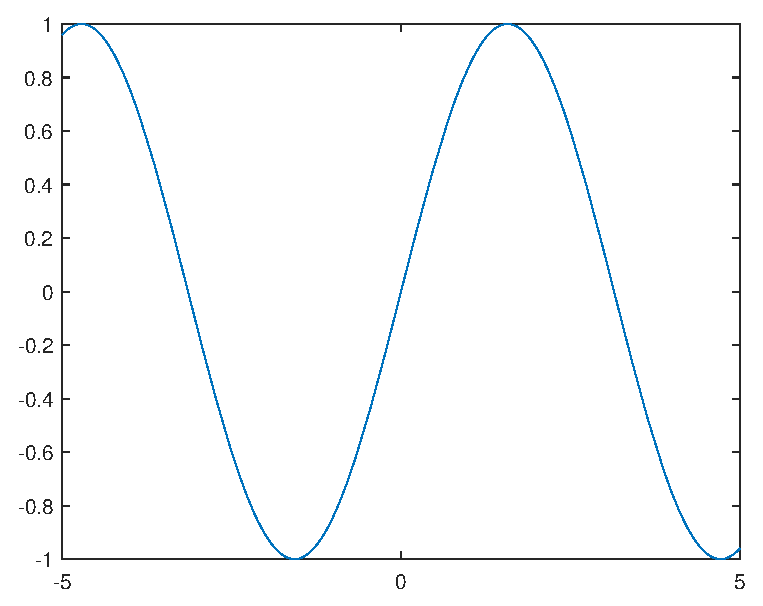
\includegraphics[width=0.5\linewidth]{image1}
\caption{Caption of Figure 1.} \label{fig:A}
\end{figure}
\end{frame}

%------------------------------------------------

\begin{frame}
\frametitle{两图并排}
\begin{figure}[htb]
\centering
\begin{minipage}{0.48\linewidth}
\centering
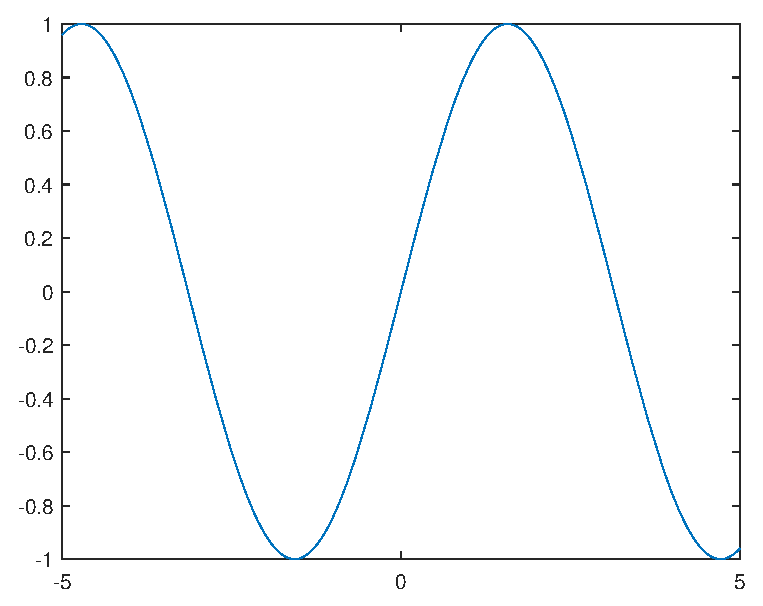
\includegraphics[width=\linewidth]{image1}
\caption{Caption of Figure 1.}
\end{minipage}\hfill
\begin{minipage}{0.48\linewidth}
\centering
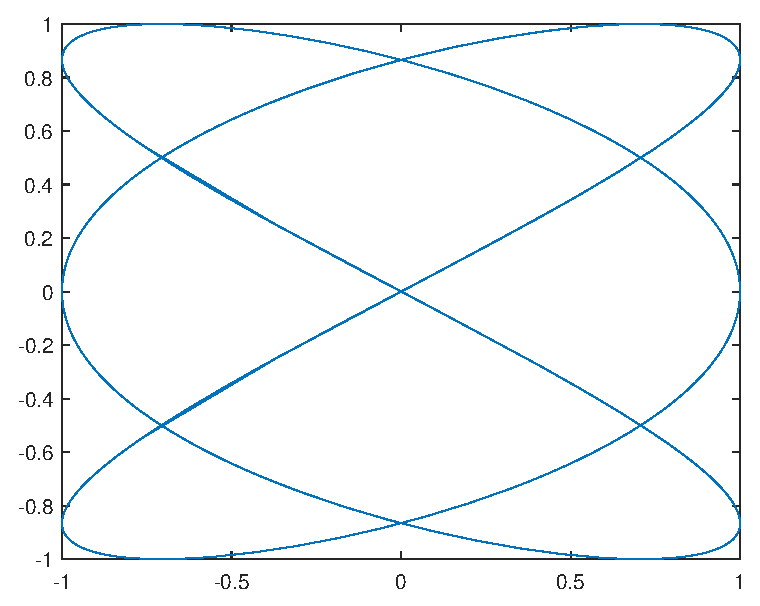
\includegraphics[width=\linewidth]{image2}
\caption{Caption of Figure 2.}
\end{minipage}
\end{figure}
\end{frame}

%------------------------------------------------
\section{参考文献}
%------------------------------------------------

\begin{frame}[fragile] % Need to use the fragile option when verbatim is used in the slide
\frametitle{Citation}
An example of the \verb|\cite| command to cite within the presentation:\\~

This statement requires citation \cite{Smith2012}. \\~

文献引用示例 \cite{LiLiu1997}, 可以修改引用文献样式.
\end{frame}

%------------------------------------------------

\begin{frame}
\frametitle{References}
\footnotesize{
\begin{thebibliography}{99} % Beamer does not support BibTeX so references must be inserted manually as below
\bibitem[Smith, 2012]{Smith2012} John Smith, Title of the publication, \emph{Journal Name}, 12(3):45--678, 2012.
\bibitem[李荣华, 1997]{LiLiu1997} 李荣华, 刘播. 微分方程数值解法. 东南大学出版社, 1997.
\end{thebibliography}
}
\end{frame}


%------------------------------------------------

\setbeamertemplate{headline}{}
\begin{frame}
%\sffamily
\begin{center}
\HUGE \textcolor[RGB]{165,3,3}{谢\quad 谢! \\[8pt]
Thank you!}
\end{center}
\end{frame}


\end{document}

